% ============================================================
% BODY -- OralGPT-Family Technical Report template
% Every paragraph below is placeholder text that explains what the
% section should contain. All numbers are placeholders, NOT results.
% Citations point to OralGPT-Family publications (see refs.bib).
% ============================================================

\section{Introduction}

This paragraph introduces the background of the report. Describe the
application setting, the data modalities involved, and the gap that the
report addresses. Previous OralGPT-Family work can be cited here, for example
the panoramic X-ray benchmark and instruction dataset~\citep{hao2025mmoral},
the versatile dental multimodal model~\citep{hao2025oralgpt-omni}, and
tool-using or agentic variants~\citep{fan2026oralgpt-plus, hao2026oralagent}.

Use a second paragraph to explain why existing approaches are insufficient
and what the key idea of this report is. Keep the description at a level
that a reader outside the immediate sub-field can follow, and point to the
overview in Figure~\ref{fig:pipeline}.

Summarise the contributions as a short list:
\begin{itemize}[leftmargin=1.2em,itemsep=2pt,topsep=3pt]
  \item \textbf{Contribution 1.} One sentence describing the first contribution (placeholder).
  \item \textbf{Contribution 2.} One sentence describing the second contribution (placeholder).
  \item \textbf{Contribution 3.} One sentence describing the released resources (placeholder).
\end{itemize}

\section{Related Work}

\textbf{Topic A.} Discuss the first line of related research and position the
report against it. Data resources and their licensing can be discussed with
reference to~\citet{hao2025oraldataset}.

\textbf{Topic B.} Discuss the second line of related research, such as
task-specific dental systems~\citep{hao2026plaquesam} or benchmark-driven
evaluation~\citep{hao2025mmoral}, and state how the present report differs.
Add further paragraphs in the same format if needed.

\section{Method}

\subsection{Overview}

Describe the overall framework in one paragraph and refer to
Figure~\ref{fig:pipeline}. Replace the placeholder figure with the framework
diagram of the report.

\begin{figure}[H] % [H] = exactly here (between 3.1 and 3.2); use [t] to let LaTeX float it
  \centering
  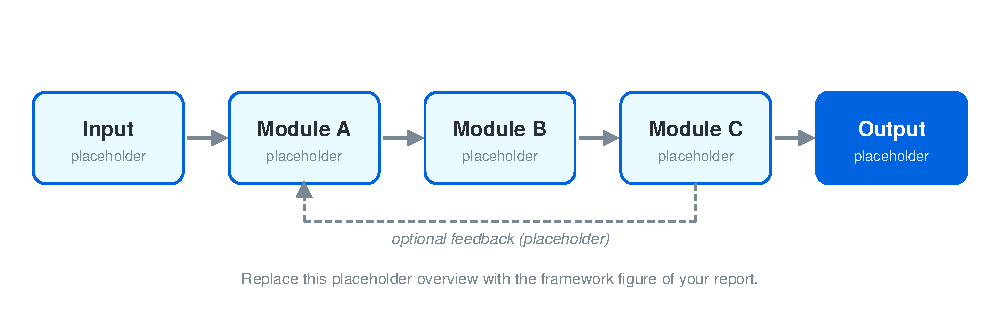
\includegraphics[width=0.98\linewidth]{assets/fig_pipeline.pdf}
  \caption{Placeholder framework overview. Replace this figure with the
  overview of your method and describe each component in one or two
  sentences.}
  \label{fig:pipeline}
\end{figure}

\subsection{Problem Formulation}

Introduce the notation used throughout the report. As a placeholder, let
$x$ denote an input sample, $\mathcal{E}_{\phi}$ an encoder and
$\mathcal{D}_{\psi}$ a decoder:
\begin{equation}
  \mathbf{h} = \mathcal{E}_{\phi}(x), \qquad
  \hat{y} = \mathcal{D}_{\psi}(\mathbf{h}).
  \label{eq:forward}
\end{equation}
For sequence outputs, the placeholder likelihood factorises as
\begin{equation}
  p_{\theta}(y \mid x) = \prod_{t=1}^{T} p_{\theta}\!\left(y_t \mid y_{<t}, x\right).
  \label{eq:likelihood}
\end{equation}

\subsection{Training Objective}

State the training objective. A generic placeholder combines a task loss with
an auxiliary term weighted by $\lambda$:
\begin{equation}
  \mathcal{L} = \mathcal{L}_{\text{task}} + \lambda\,\mathcal{L}_{\text{aux}},
  \label{eq:objective}
\end{equation}
where $\mathcal{L}_{\text{task}}$ is the negative log-likelihood of
Equation~\eqref{eq:likelihood}. Describe the training stages, data mixture
and optimisation settings here, and move full details to
Appendix~\ref{app:details}.

\section{Experiments}

\subsection{Experimental Setup}

Describe the datasets, benchmarks, baselines and evaluation metrics. State
how splits are constructed and how the main hyperparameters are chosen.

\begin{table}[t]
  \centering
  \footnotesize
  \caption{Placeholder main results. Replace the rows and columns with the
  models and benchmarks of your report. \textbf{All values are placeholders.}}
  \label{tab:main}
  \begin{tabularx}{\linewidth}{>{\raggedright\arraybackslash}Xcccc}
    \toprule
    Model & Benchmark A & Benchmark B & Benchmark C & Benchmark D \\
    \midrule
    Baseline-1              & 58.2 & 49.4 & 63.1 & 55.7 \\
    Baseline-2              & 66.5 & 58.9 & 69.8 & 63.4 \\
    OralGPT-Family (ours)   & \textbf{81.3} & \textbf{74.6} & \textbf{86.2} & \textbf{79.5} \\
    \bottomrule
  \end{tabularx}
\end{table}

\subsection{Main Results}

Summarise the main results with reference to Table~\ref{tab:main} and
Figure~\ref{fig:benchmark}. Report the key comparisons in one or two
sentences each and relate them to the design choices of
Equation~\eqref{eq:objective}.

\begin{figure}[t]
  \centering
  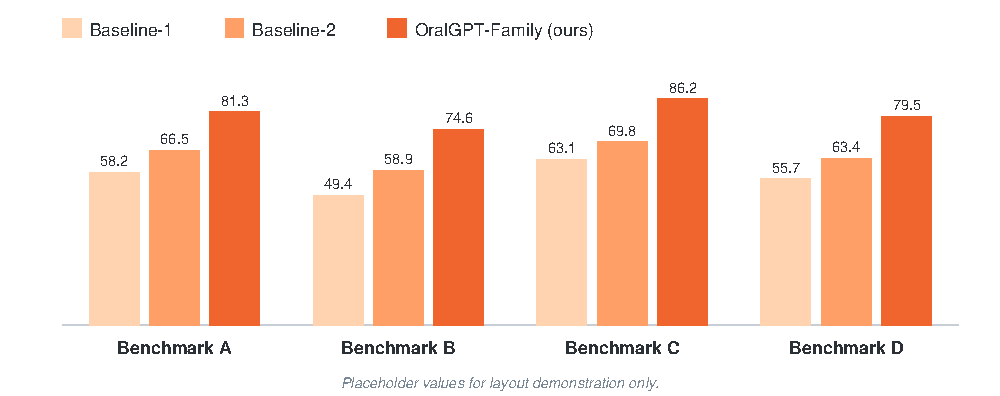
\includegraphics[width=0.8\linewidth]{assets/fig_results.pdf}
  \caption{Placeholder benchmark comparison. Replace this chart with the
  results of your report; the values shown are placeholders.}
  \label{fig:benchmark}
\end{figure}

\subsection{Ablation Study}

Describe the ablation experiments: which components are removed or varied,
and what the placeholder outcome would indicate. Larger ablation tables can be
moved to Appendix~\ref{app:results}.

\section{Conclusion}

Summarise the report in one paragraph: what was proposed, how it was
evaluated, and what is released. State the main limitations (for example data
coverage and the need for clinical validation) and, optionally, directions for
future work within the OralGPT-Family.

\bibliographystyle{plainnat}
\bibliography{refs}
